\label{chapter:metodo}

\par
Com a grande quantidade de dados que são armazenados pelas universidades de seus candidatos ao vestibular, muitas delas não sabem em como utilizar esses dados para benefício próprio. Com base nesses dados armazenados, especificamente os dados dos candidatos que prestaram o vestibular, se pretende aplicar a mineração de dados educacional, com o objetivo de extrair o conhecimento dessa base para saber quais fatores que afetam o desempenho desse candidato em sua nota do vestibular. Neste contexto o trabalho proposto segue as seguintes etapas para se alcançar esse objetivo conforme a Figura 18.

\par
\begin{figure}[!htp]
	\begin{center}
    \caption{\label{fig:waveform_fig} Diagrama do método proposto.}
	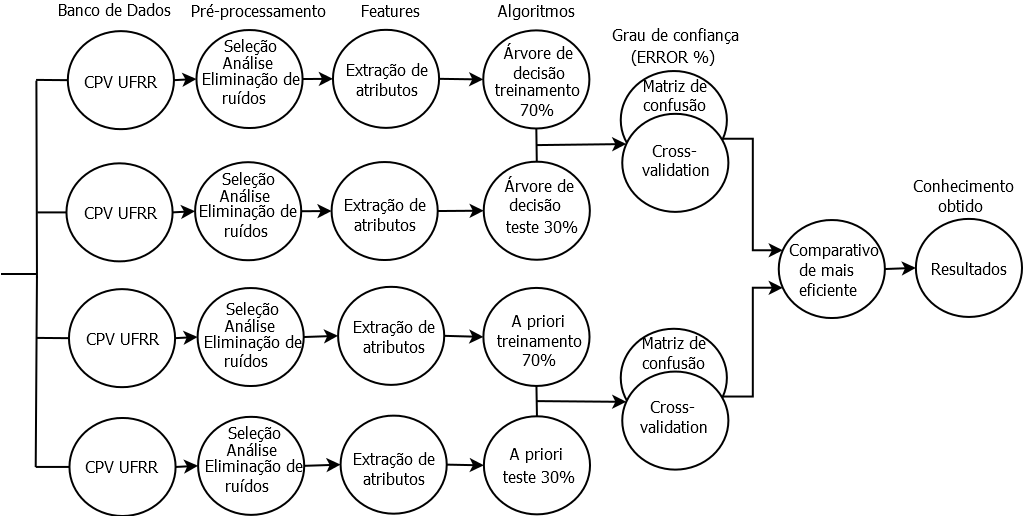
\includegraphics[scale=0.45]{Figuras/Caso_de_uso_metodo_TCC1.png}
	\end{center}
    \legend{Fonte: Própria}
\end{figure}

\par
Para a fase de pré-processamento (uma das etapas do KDD demonstrado em conceitos de definições), será analisado o banco de dados do vestibular da Universidade Federal de Roraima (UFRR) do ano de 2017 fornecido pela Comissão Permanente de Vestibular (CPV), que está encarregada de gerenciar os dados geral dos candidatos inscritos. Para formar a base de dados onde será aplicado a mineração, estará sendo feita a junção dos dados dos questionários socioeconômico que contém no total de 37 questões e os dados de cadastro geral que são realizados pelos candidatos durante a etapa de inscrição.


\par
Como em todo banco de dados é normal encontrar inconsistência de dados, como ruídos, itens de dados em branco, valores absurdos e erros de digitação, para garantir a qualidade dos dados, serão necessário corrigir esses problemas para que na hora da mineração não ocorra nenhum erro ou que tenha algum resultado incoerente. Tambám será necessário ser feito a eliminação de atributos repetidos assim como dados irrelevantes para a pesquisa e dos dados de candidatos que não compareceram para prestar o vestibular.

\par
Na extração das \textit{features}, pode se ter como base os mesmos atributos que foram selecionados no trabalho de \citeonline{Simon2017}, onde, dentre os 25 atributos apresentados em sua base de dados, depois de alguns testes, apenas 9 delas foram consideradas como relevante para o seu trabalho. Com esses atributos selecionados por \citeonline{Simon2017} será feito um comparativo com as \textit{features} selecionadas pelos algoritmos de seleção de atributos da ferramenta WEKA, para escolher entre elas os atributos mais relevantes que servirão para a mineração e associação de dados deste trabalho.


\par
Depois de selecionar e transformar a base de dados em um formato apropriado, será aplicado a técnica de mineração de árvore de decisão para a análise de dados dos candidatos, a escolha desse método foi pelo seguinte motivo, que segundo \citeonline{Simon2017}, esta técnica serve como um sistema de suporte a decisão, que é utilizado para aprender funções de classificação que mostra o valor de uma variável dependente por meio de dados de variáveis independentes fornecidos. Para alguns autores a técnica de árvore de decisão é considerada uma das abordagens mais poderosas em mineração de dados e descoberta do conhecimento. Contudo, durante o desenvolvimento deste trabalho também serão avaliados outros algoritmos de aprendizagem de máquina, visando assim encontrar uma melhor acurácia do modelo gerado.

\par
Dentre os algoritmos de árvore de decisão, foi optado em utilizar o algoritmo J48, pois, segundo \citeonline{Simon2017} e \citeonline{Martinhago2005} que utilizaram o mesmo algoritmo, o algoritmo J48 gera a árvore de decisão e a transforma em regras de classificação, além de que na literatura é bastante utilizado em aplicações educacionais. O software utilizado para a tarefa de classificação e mineração dos dados é o WEKA que já tem o algoritmo J48 disponível nele, que segundo \citeonline{Simon2017} o WEKA é utilizado a muito tempo em pesquisas que envolvem mineração de dados, sendo aceito amplamente tanto em empresas como academias tendo uma comunidade muito grande que ainda esta ativa.

\par
A ferramenta WEKA foi escolhida pelo motivo de possuir todos os classificadores implementados, além de fornecer outras funcionalidades para pré-processamento, classificação, regressão, agrupamentos, regras de associação, visualização e entre outros \cite{Camilo2009}. Segundo \citeonline{Amaral2016} algumas vantagens de se utilizar o software WEKA é que ela é uma ferramenta gratuita, madura que está disponível desde os anos 90 com inúmeros algoritmos que executam diversas tarefas de aprendizagem de máquina e possui uma interface gráfica interativa, fácil de manusear sem a necessidade de se digitar códigos. 

\par
Para saber a eficiência do algoritmo de árvore de decisão na base de dados proposto, será aplicado a técnica de associação de dados utilizando o algoritmo a priori na mesma base de dados, para saber a eficiência entre as duas através de uma comparação dos seus resultados. Segundo \citeonline{Librelotto2014} o algoritmo a priori pode executar várias passagens pelo banco além de trabalhar com um número grande de atributos, tendo como resultado várias alternativas combinadas entre eles através das buscas sucessivas em toda a base de dados. O motivo de se ter essas buscas sucessivas é que ele usa o mesmo raciocínio de dividir para conquistar, com intuito de encontrar regras de associação para todos os atributos possíveis, executando um processo de indução de regras para todas as combinações possíveis de atributos.


\par
Para avaliar os resultados obtidos depois de todos os testes, será utilizado a métrica de avaliação de modelo matriz de confusão e resultados da aplicação \textit{crossvalidation} para determinar se o resultado previsto corresponde ao resultado real. Segundo os trabalhos \citeonline{Simon2017} e \citeonline{Silva2014} que possui base semelhante que será utilizado nesse TCC, nota-se que acurácia resultante para o modelo é aproximadamente a partir de 70\%, ou seja, estaremos utilizando esta porcentagem de acurácia para avaliar os resultados que serão obtidos. Ao final dessas etapas, a partir dos resultados e conhecimento extraído, se espera gerar um perfil para poder encontrar os principais fatores que influencia o bom ou o mau desempenho das notas dos candidatos para o vestibular.

\par 
Através da mineração de dados, com as regras geradas se pode ter como conhecimento relevante para futuras ações da UFRR, referente ao perfil dos candidatos que prestaram seletivo para o vestibular. Como este trabalho tem como intuito uma análise mais profunda dos fatores que afetam o desempenho dos vestibulandos, para poder observar os padrões que tem mais em comum entre eles, pode-se considerar que esta análise está voltada para o desenvolvimento social dos candidatos. Com isso, com os resultados obtidos, pode servir como contribuição para o MEC avaliar em como está indo a sua estratégia do plano de ensino para as escolar públicas, federais e privadas e para o Ministério de Desenvolvimento Social (MDS) para tentar amenizar os possíveis problemas socioeconômico encontrados.

